\documentclass[aspectratio=169,11pt]{beamer}
\makeatletter
\input{../../templates/dune-professional/beamerthemeDUNEProfessional.sty}
\makeatother
\title{Ground shakes}
\author{Manuel Arroyave}
\date{27 October 2026}

% Figures need plain captions, not the shared component's "Diagram" prefix.
\renewcommand{\DuneDiagramCaption}[1]{%
  {\small\color{DuneText}#1\par}}
\newcommand{\PlotNote}[1]{%
  \smallskip{\footnotesize\color{DuneTextMuted}#1\par}}

\begin{document}

\begin{frame}{Ground shakes: a repeatable electrical response}
  \framesubtitle{ProtoDUNE-HD · Manuel Arroyave · Analysis through 27 October 2026}
  \begin{columns}[T,onlytextwidth]
    \begin{column}{0.39\textwidth}
      \textbf{We checked seven runs.}\par
      \smallskip
      {\small
      \renewcommand{\arraystretch}{1.16}
      \begin{tabularx}{\linewidth}{@{}Xrr@{}}
        \toprule
        2024 data & Run & Events \\
        \midrule
        July & 27938 & 6 \\
             & 27951 & 19 \\
        October & 30201 & 44 \\
                & 30202 & 83 \\
        November & 32730 & 1 \\
                 & 32731 & 716 \\
                 & 32739 & 662 \\
        \midrule
        Total & & 1,531 \\
        \bottomrule
      \end{tabularx}}
    \end{column}
    \begin{column}{0.56\textwidth}
      \textbf{We used charge and PDS data.}\par
      {\small TPC: charge readout. PDS: photon detector readout.\par
      Slow controls (SC): 34 monitors; 7.74 million samples.}\par
      \medskip
      \textbf{Charge test: 1,516 possible shakes.}\par
      {\small Five records did not pass the test; ten lacked usable charge data.}\par
      \medskip
      \begin{itemize}
        \item Same slow charge shape, opposite signs.
        \item Electrical pattern transfers between runs.
        \item No robust SC correlation found in our test.
      \end{itemize}
    \end{column}
  \end{columns}
  \PlotNote{Selected records; automatic labels need review. The initiating source is still unknown.}
\end{frame}

\begin{frame}{A PDS pulse comes before the large disturbance}
  \framesubtitle{Run 27938 · event 20576 · APA1 charge and continuous PDS readout}
  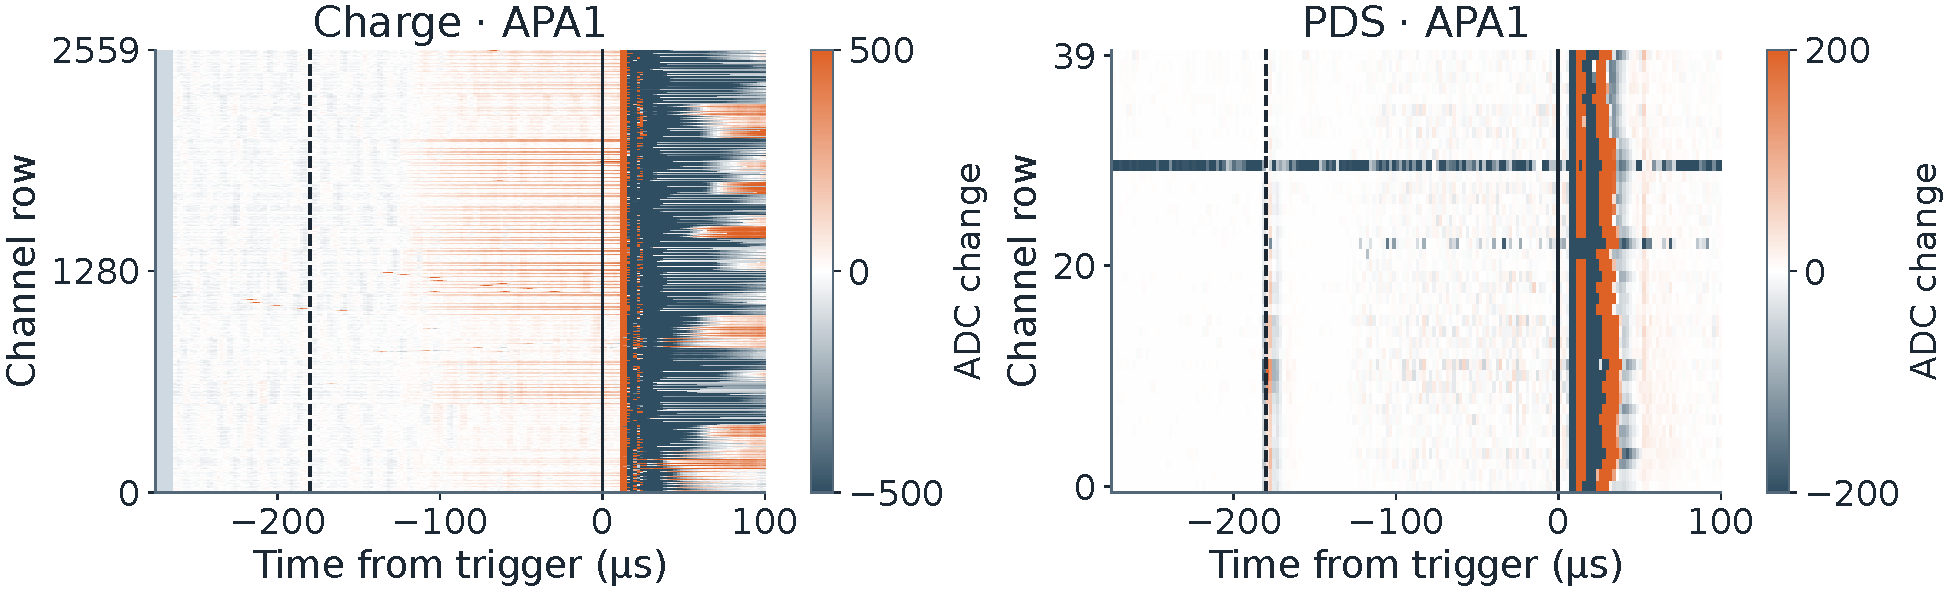
\includegraphics[width=\textwidth]{figures/01-charge-and-pds.pdf}
  \DuneDiagramCaption{Each row is one channel. Blue is below baseline; orange is above it.
    The dashed line marks an early PDS pulse, about 180\,$\mu$s before the trigger (0).
    Both systems then show a large disturbance. Grey means unrecorded.}
  \PlotNote{ADC counts are raw signal units; $\mu$s means millionths of a second.
    Colour limits clip large signals. Recorded timing; electronics delays uncorrected.}
\end{frame}

\begin{frame}{The slow charge signals move in opposite directions}
  \framesubtitle{APA1 and APA2 are the two charge-readout assemblies used here}
  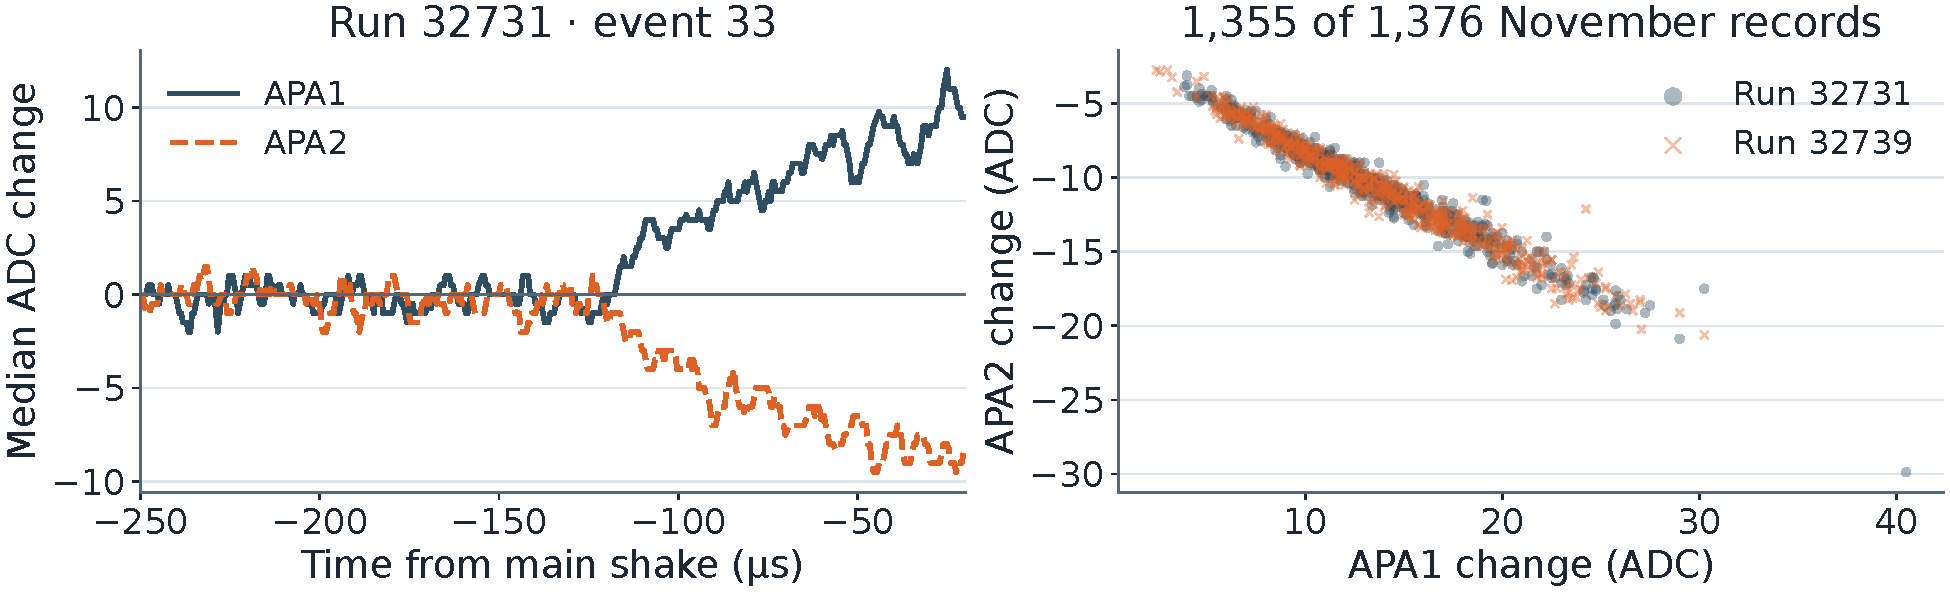
\includegraphics[width=\textwidth]{figures/02-opposite-charge-signs.pdf}
  \DuneDiagramCaption{\textbf{Left:} one event. APA1 rises while APA2 falls before the main shake.
    \textbf{Right:} one dot per event. This pattern is clear in 1,355 of 1,376 November records.}
  \PlotNote{Median shape correlation after reversing APA2: 0.964 and 0.970 in the two runs.
    A score of 1 means the same shape.}
\end{frame}

\begin{frame}{Disconnected PDS inputs also carry pulses}
  \framesubtitle{Run 32731 · event 33 · selected pulse 183.296\,$\mu$s before the main shake}
  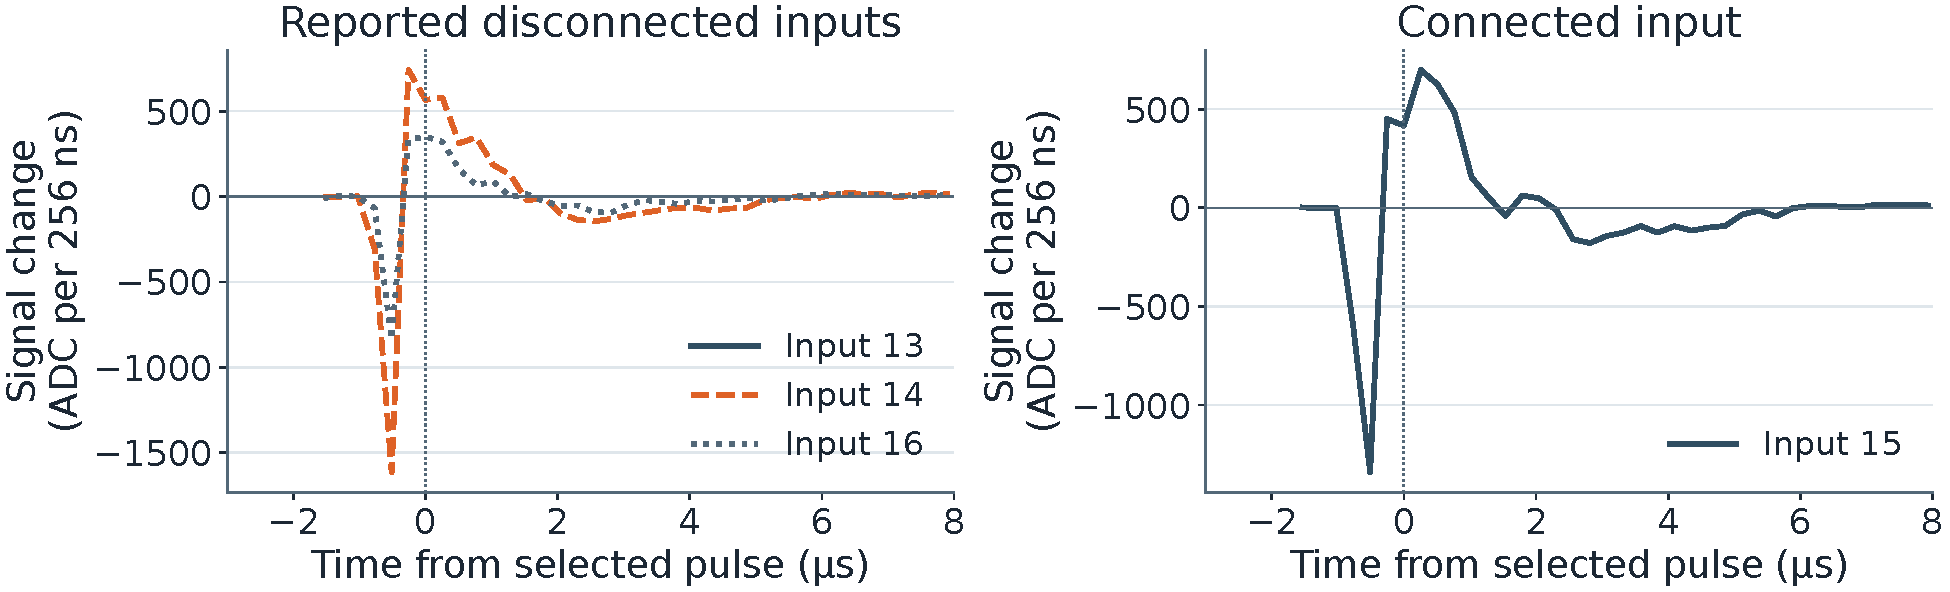
\includegraphics[width=\textwidth]{figures/03-disconnected-inputs.pdf}
  \DuneDiagramCaption{\textbf{Left:} inputs 13, 14 and 16 were reported disconnected from the sensors.
    \textbf{Right:} connected input 15 responds at the same time.
    This supports electrical pickup. It does not identify what started the pulse.}
  \PlotNote{Each line shows signal change in 256 ns steps. The reported disconnections still need run-specific confirmation.}
\end{frame}

\begin{frame}{The electrical pattern transfers to another run}
  \framesubtitle{Fit trained on run 32731; all run 32739 events excluded from training}
  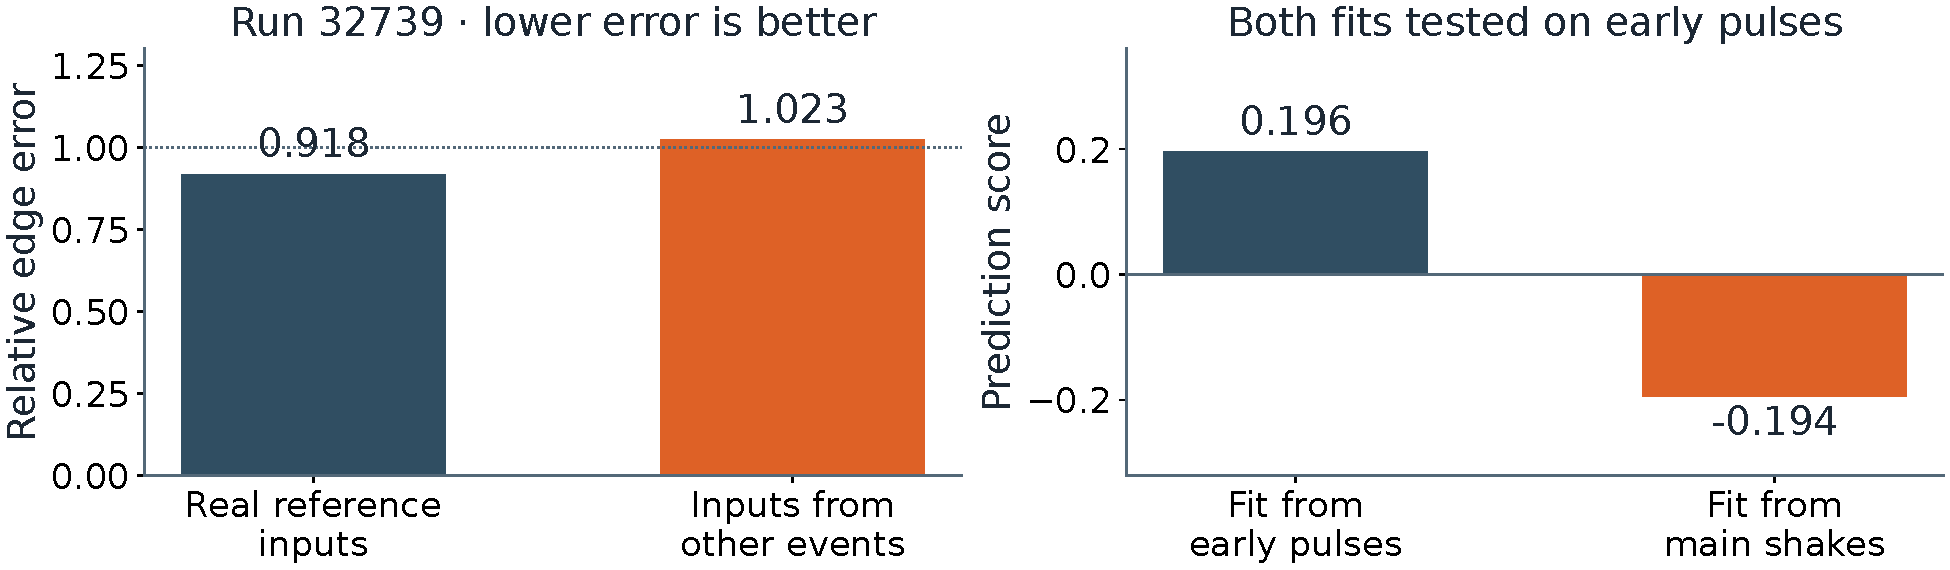
\includegraphics[width=\textwidth]{figures/07-cross-run-electrical.pdf}
  \DuneDiagramCaption{\textbf{Left:} the real disconnected-input signals give less error than inputs from other events.
    \textbf{Right:} a fit trained on the main shake fails on early pulses.
    One simple response does not describe both stages.}
  \PlotNote{A positive score beats a zero-change guess. Large pulses dominate the combined score;
    the median score per event is only 0.022. This is not a light/electrical fraction.}
\end{frame}

\begin{frame}{The response depends on the electronics channel}
  \framesubtitle{Same early-pulse fit; tested on run 32739}
  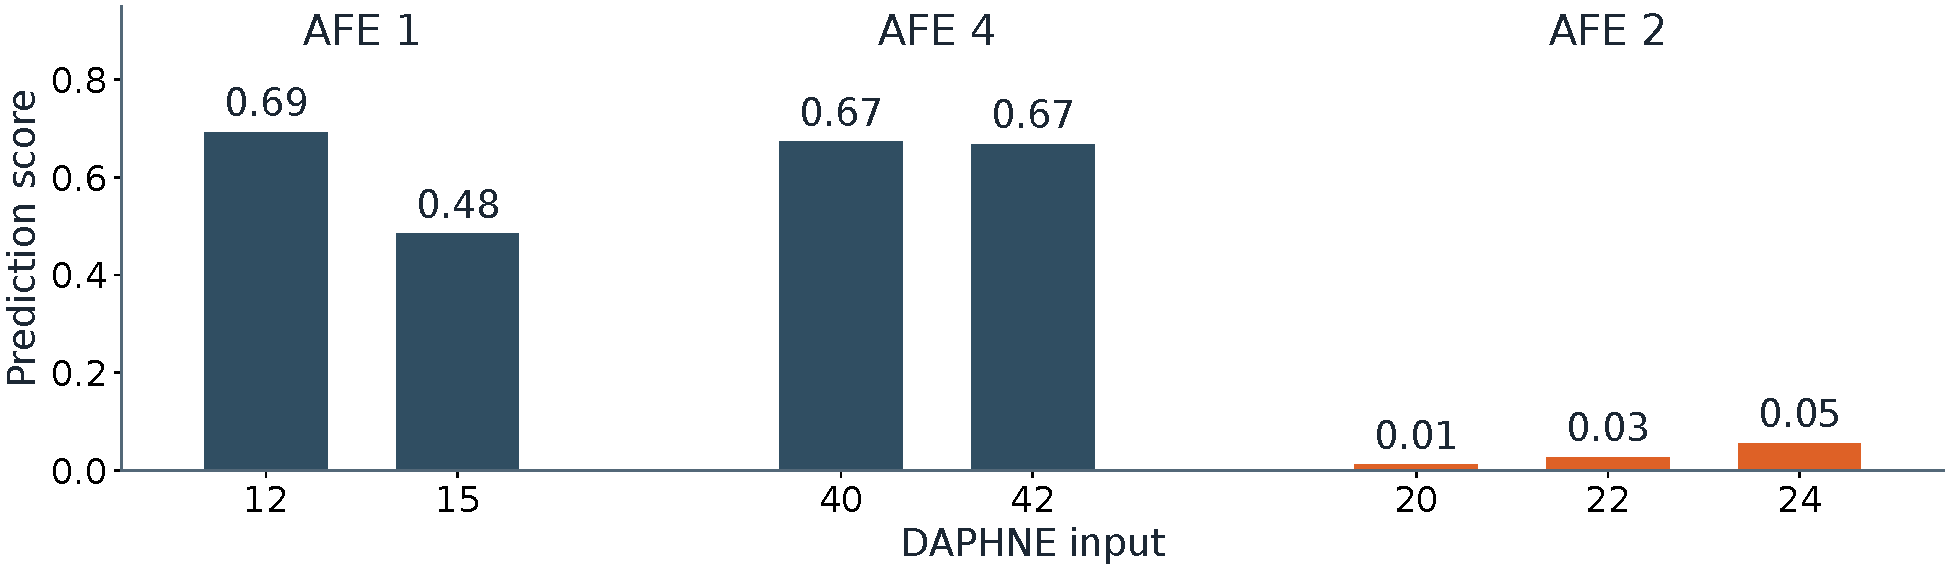
\includegraphics[width=\textwidth]{figures/08-electronics-groups.pdf}
  \DuneDiagramCaption{Each bar is one connected input. Taller bars mean better prediction from the disconnected inputs.
    Inputs 12/15 and 40/42 are well predicted. Inputs 20/22/24 remain largely unexplained.}
  \PlotNote{An AFE is an eight-channel front-end chip. Score: 0 = no improvement; 1 = exact prediction.
    The unequal response constrains the circuit model.}
\end{frame}

\begin{frame}{We found no unique charge--light match}
  \framesubtitle{Early PDS pulses compared with later charge features · November runs}
  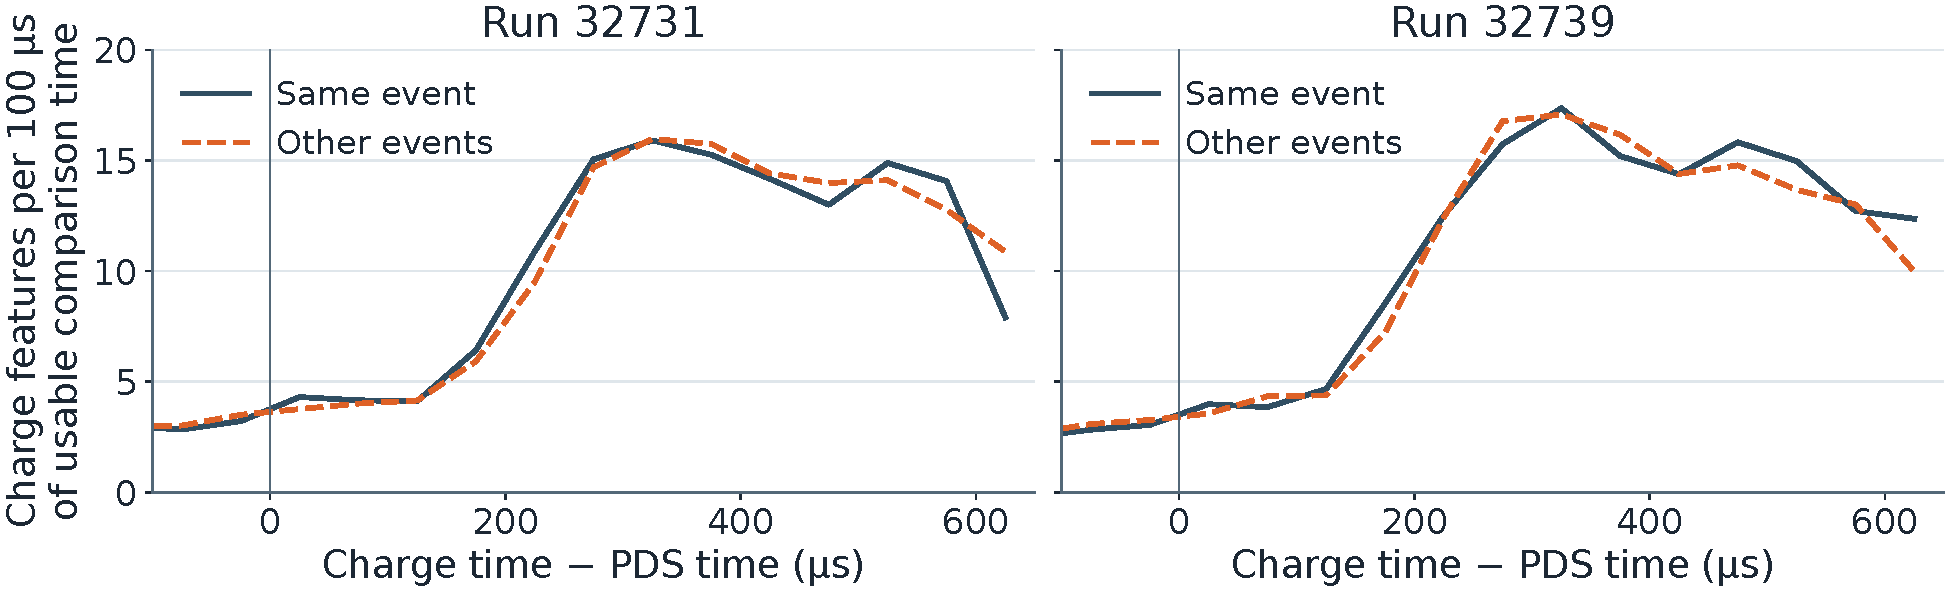
\includegraphics[width=\textwidth]{figures/05-charge-light-timing.pdf}
  \DuneDiagramCaption{The horizontal axis is charge time minus PDS time.
    Blue uses pulses from the same event; dashed orange uses pulses from other events.
    Both show the peak near 325\,$\mu$s. That peak alone does not link a PDS pulse to a charge track.}
  \PlotNote{Counts account for recorded comparison time. Pulses are swapped within the same run, file and assembly.
    This is not a normal-running background test.}
\end{frame}

\begin{frame}{We found no robust SC--waveform correlation}
  \framesubtitle{32 testable monitors × 3 measurements · Runs 32731 and 32739 · Two ground monitors too sparse}
  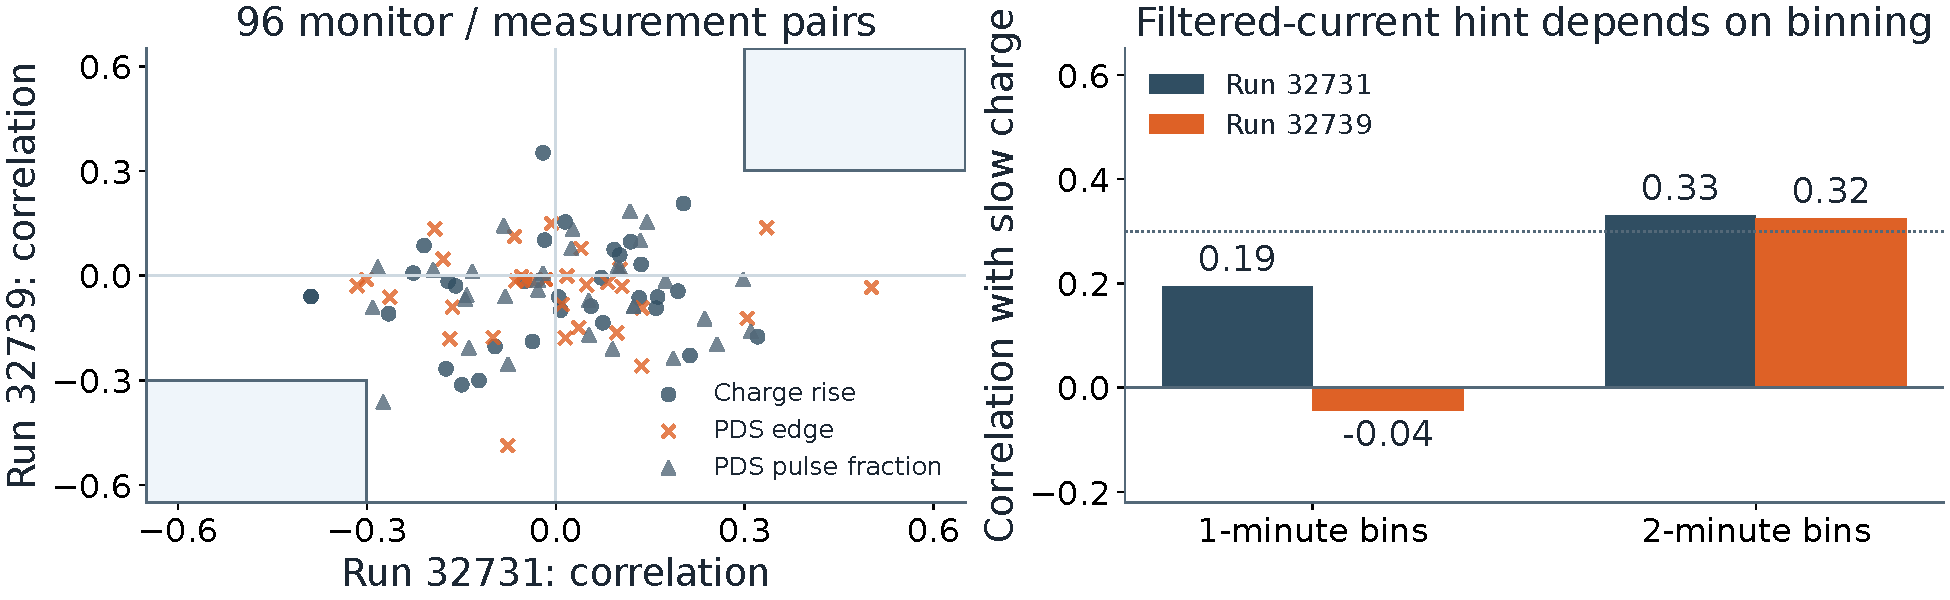
\includegraphics[width=\textwidth]{figures/09-SC-correlation.pdf}
  \DuneDiagramCaption{\textbf{Left:} each dot tests one monitor against one waveform measurement.
    Shaded corners mark a repeat in both runs; none qualify with one-minute bins.
    \textbf{Right:} a weak filtered-current hint depends on binning and does not survive the other checks.}
  \PlotNote{Test: magnitude at least 0.30, with the same sign in both runs; file and time-trend adjusted.
    This tests waveform changes within selected shakes, not shake rate or fast transients.}
\end{frame}

\begin{frame}{Next: tracks, controls and the electrical path}
  \DuneCompactColorBlock{paper}{USE THE SAVED DATA}{Fit charge tracks for 348 unexplained pulse windows}
    {Check the run geometry and timing. Compare whole charge tracks with each possible light pulse.}
  \medskip
  \DuneCompactColorBlock{sky}{ADD MATCHED CONTROLS}{Measure the excess and false-alarm rate}
    {Find records without shakes using the same boards, gains and triggers, with measured live time.}
  \medskip
  \DuneCompactColorBlock{coral}{CHECK THE HARDWARE}{Test which electrical path gives this channel pattern}
    {Confirm wiring and AFE settings. Measure fast supply, ground and reference signals.}
  \PlotNote{No candidate has a full 4 ms of pre-shake PDS data.
    The SC export contains no direct DAPHNE supply monitors.}
\end{frame}

\appendix
\begin{frame}{Backup: July voltage records}
  \framesubtitle{Eleven July candidates; ten occur in one 26-second burst}
  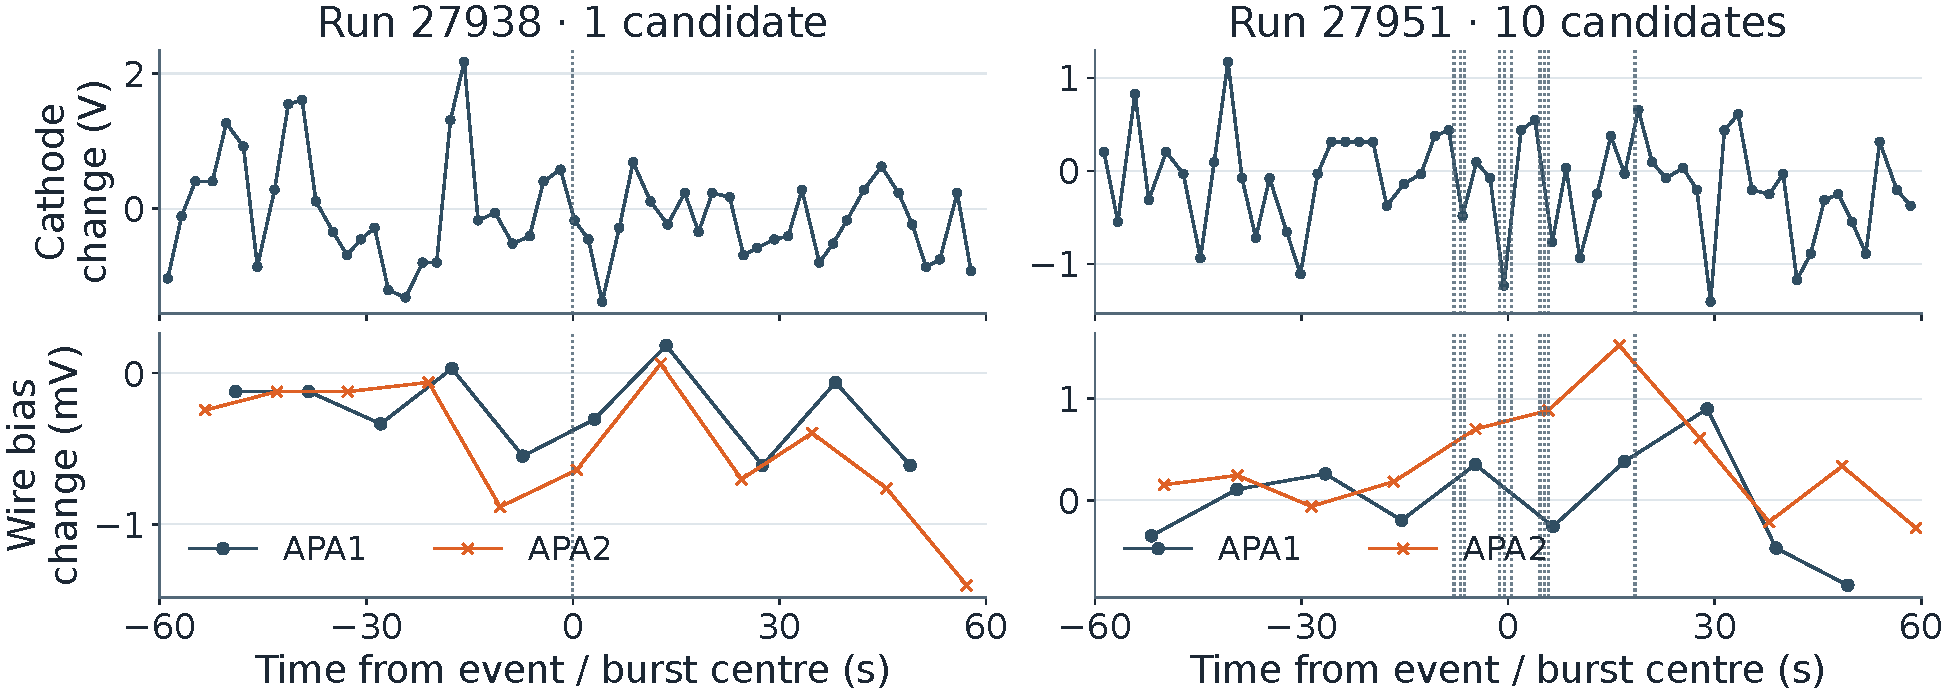
\includegraphics[width=\textwidth]{figures/06-july-voltage.pdf}
  \DuneDiagramCaption{\textbf{Top:} cathode voltage change. \textbf{Bottom:} wire-bias change.
    Dots are archived samples; vertical marks are shake candidates.
    Sampling every 2--11 seconds cannot rule out a brief discharge.}
  \PlotNote{Changes are relative to the preceding baseline: about 176 kV for the cathode and $-370$ V for the wire bias.}
\end{frame}

\begin{frame}{Backup: early PDS gives weak charge predictions}
  \framesubtitle{Trained on run 32731; tested on unused run 32739 events · Lower bars are better}
  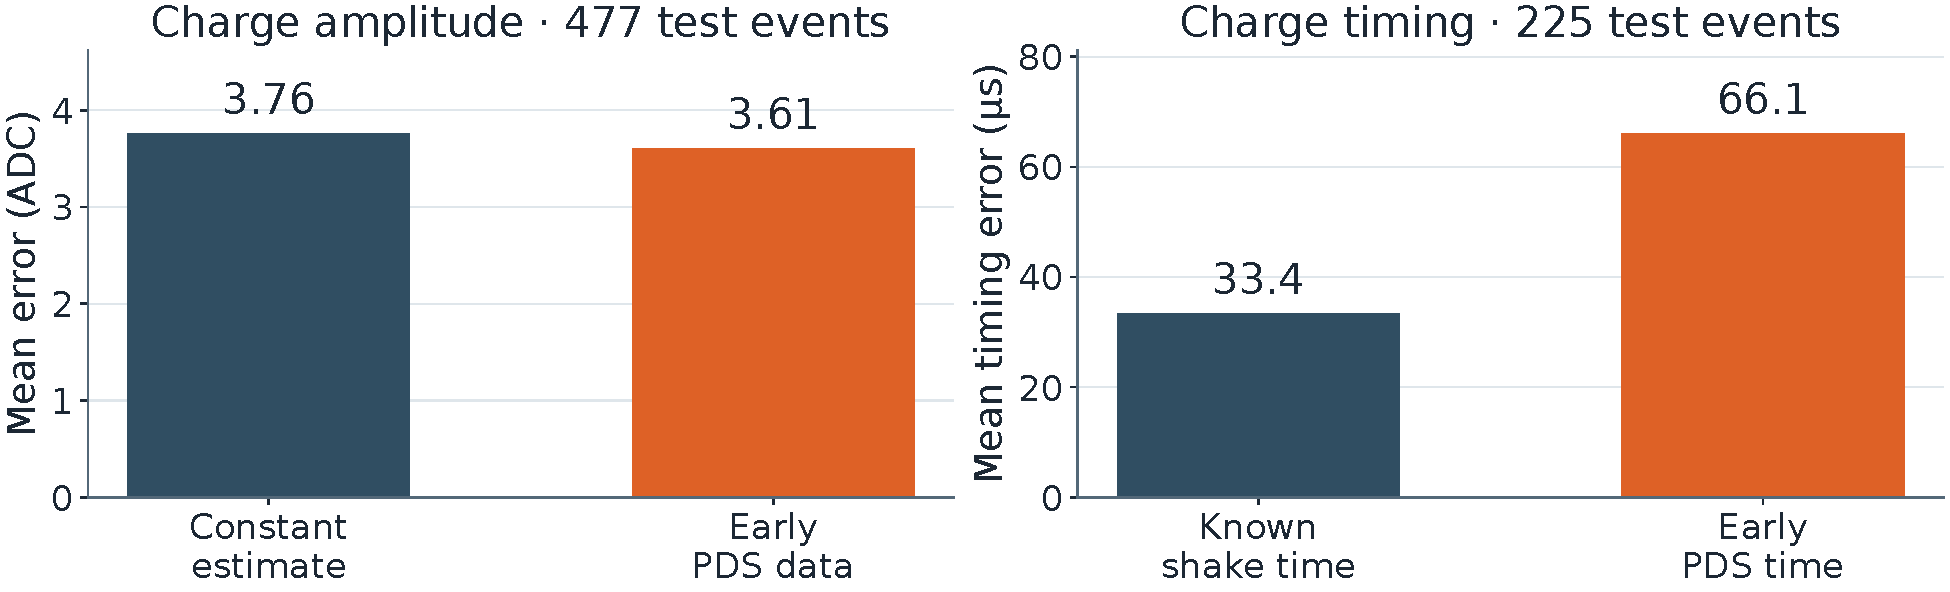
\includegraphics[width=\textwidth]{figures/04-pds-prediction.pdf}
  \DuneDiagramCaption{\textbf{Left:} early PDS data reduce the charge-amplitude error by only 4.1\%.
    \textbf{Right:} the early pulse predicts the 2 ADC charge crossing less accurately than the known main-shake time.
    These checks use saved events.}
  \PlotNote{This tests variation within selected shakes. It does not test whether PDS can predict that a shake will occur.}
\end{frame}

\end{document}
